\section{Explications basées sur des exemples}

Les méthodes d'explication basées sur des exemples sélectionnent des instances particulières de l'ensemble de données pour expliquer le comportement des modèles de machine learning ou pour expliquer la distribution sous-jacente des données.
Les explications basées sur des exemples sont pour la plupart indépendantes des modèles et ont un sens si nous pouvons représenter une instance des données d'une manière humainement compréhensible.

\subsection{Explications Contrefactuelles}
Une explication contrefactuelle d'une prédiction décrit le plus petit changement apporté aux valeurs des variables qui modifie la prédiction vers une prédiction prédéfinie. Cette méthode est agnostique du modèle, car elle ne fonctionne qu'avec les entrées et sorties du modèle. Elle pourrait aussi bien être située dans le chapitre sur les méthodes agnostiques des modèles, car l'interprétation peut être exprimée comme un résumé des différences dans les valeurs des variables (``changer les variables A et B pour changer la prédiction''). Cependant, une explication contrefactuelle est en elle-même une nouvelle instance, donc elle se trouve dans ce chapitre.

Les contrefactuels sont des explications acceptées par les humains, car elles sont contrastées et parce qu'elles sont sélectives, c'est-à-dire qu'elles se concentrent généralement sur un petit nombre de changements de variables. Cependant, les contrefactuels souffrent de l'effet de `Rashomon', Rashomon est un film japonais dans lequel le meurtre d'un Samouraï est raconté par différentes personnes. Chacune des histoires explique également bien le résultat, mais les histoires se contredisent.

\subsubsection{Génération d'Explications Contrefactuelles}
Wachter et al. suggèrent de minimiser la perte suivante :
\[
L(x,x^\prime,y^\prime,\lambda)=\lambda\cdot(\hat{f}(x^\prime)-y^\prime)^2+d(x,x^\prime)
\]
Le premier terme est la distance quadratique entre la prédiction du modèle pour le contrefactuel \(x'\) et le résultat souhaité \(y'\), que l'utilisateur doit définir à l'avance.
Le deuxième terme est la distance \(d\) entre l'instance \(x\) à expliquer et le contrefactuel \(x'\).

La fonction de distance \(d\) est définie comme la distance de Manhattan pondérée par l'écart médian absolu inverse (MAD) de chaque variable.
\[
d(x,x')=\sum_{j=1}^p\frac{|x_j-x'_j|}{MAD_j}
\]
La distance totale est la somme de toutes les distances spécifiques à chaque variable \(p\), c'est-à-dire les différences absolues des valeurs des variables entre l'instance \(x\) et le contre-factuel \(x'\).

Les distances spécifiques à chaque variable sont mises à l'échelle par l'inverse de l'écart médiane absolue de la variable \(j\) sur l'ensemble de données défini comme suit:
\[
MAD_j=\text{médiane}_{i\in\{1,\ldots,n\}}(|x_{i,j}-\text{médiane}_{l\in\{1,\ldots,n\}}(x_{l,j})|)
\]
Pour minimiser la fonction de perte, tout algorithme d'optimisation approprié peut être utilisé, comme le Nelder-Mead. Si vous avez accès aux gradients du modèle d'apprentissage automatique, vous pouvez utiliser des méthodes basées sur le gradient telles qu'ADAM.

L'instance \(x\) à expliquer, la sortie souhaitée \(y'\) et le paramètre de tolérance \(\epsilon\) doivent être fixés à l'avance. La fonction de perte est minimisée pour \(x'\) et le contre-factuel \(x'\) (localement) optimal est renvoyé tout en augmentant \(\lambda\) jusqu'à ce qu'une solution suffisamment proche soit trouvée (= dans la tolérance du paramètre):
\[
\arg\min_{x'}\max_{\lambda}L(x,x',y',\lambda).
\]
En somme, la recette pour produire les contre-factuels est simple :
\begin{enumerate}
    \item Sélectionner une instance \(x\) à expliquer, le résultat souhaité \(y'\), une tolérance \(\epsilon\) et une valeur initiale faible pour \(\lambda\).
    \item Échantillonner une instance aléatoire comme contre-factuel initial.
    \item Optimiser la perte avec le contre-factuel initialement échantillonné comme point de départ.
    \item Tant que \(|\hat{f}(x')-y'|\)>\(\epsilon\):
    \begin{enumerate}
        \item Augmenter \(\lambda\).
        \item Optimiser la perte avec le contre-factuel actuel comme point de départ.
        \item Renvoyer le contre-factuel qui minimise la perte.
    \end{enumerate}
    \item Répéter les étapes 2 à 4 et renvoyer la liste des contre-factuels ou celui qui minimise la perte.
\end{enumerate}

La méthode proposée présente certains inconvénients. Elle ne prend en compte que les critères: produire des contre-factuels avec seulement quelques changements de variables et des valeurs de variables probables . Elle n'encourage pas les solutions "sparse" puisque l'augmentation de 10 variables de 1 donnera la même distance à \(x\) que l'augmentation d'une variable de 10. Les combinaisons de variables irréalistes ne sont pas pénalisées.


\subsubsection{Avantages}
\begin{itemize}
    \item L'interprétation des explications contrefactuelles est très claire.
    \item Aucune hypothèse supplémentaire et pas de "magie" en arrière-plan.
    \item La méthode fonctionne aussi avec des systèmes qui n'utilisent pas l'apprentissage automatique.
    \item Facilité de mise en œuvre, car il s'agit essentiellement d'une fonction de perte qui peut être optimisée avec des bibliothèques d'optimisation standard.
\end{itemize}

\subsubsection{Inconvénients}
\begin{itemize}
    \item Pour chaque instance, vous trouverez généralement plusieurs explications contrefactuelles (effet Rashomon).
    \item Aucune garantie qu'une instance contrefactuelle soit trouvée.
    \item La méthode ne gère pas bien les variables catégorielles avec de nombreux niveaux différents.
    \item Manque d'une implémentation logicielle générale.
\end{itemize}



\subsection{Exemples Adversaires}
Un exemple adverse est une instance avec de petites perturbations intentionnelles de variables qui amènent un modèle d'apprentissage automatique à faire une fausse prédiction. Les exemples adversaires sont des contre-factuels avec l'objectif de tromper le modèle et non pas de l'interpréter.
La plupart des approches suggèrent de minimiser la distance entre l'exemple adverse et l'instance à manipuler, tout en déplaçant la prédiction vers le résultat (adversaire) souhaité.
Ces exemples adversaires sont générés en minimisant la fonction suivante par rapport à \( r \):
\[
\text{loss}(\hat{f}(x+r),l)+c\cdot|r|
\]

Dans cette formule, \( x \) est une image (représentée comme un vecteur de pixels), \( r \) sont les changements apportés aux pixels pour créer une image adverse (\( x+r \) produit une nouvelle image), \( l \) est la classe de résultat souhaitée, et le paramètre \( c \) est utilisé pour équilibrer la distance entre les images et la distance entre les prédictions.
La première terme mesure la distance entre l'issue prédite de l'exemple adverse et la classe désirée \( l \), le second terme mesure la distance entre l'exemple adverse et l'image originale.
Cette formulation est presque identique à la fonction de perte pour générer des \hyperref[counterfactual]{explications contre-factuelles}.
Des contraintes supplémentaires pour \( r \) garantissent que les valeurs des pixels restent entre 0 et 1.
Les auteurs suggèrent de résoudre ce problème d'optimisation avec un L-BFGS à boîtes, un algorithme d'optimisation qui fonctionne avec les gradients.

\subsubsection{Méthode du Fast Gradient Sign}

Goodfellow et al. (2014) ont inventé la méthode du signe du gradient rapide pour générer des images adverses. Cette méthode utilise le gradient du modèle sous-jacent pour trouver des exemples adverses. L'image originale $x$ est manipulée en ajoutant ou en soustrayant une petite erreur $\epsilon$ à chaque pixel. Le choix entre l'ajout ou la soustraction de $\epsilon$ dépend du signe du gradient pour un pixel donné, qu'il soit positif ou négatif. Ajouter des erreurs dans la direction du gradient signifie que l'image est intentionnellement modifiée de manière à ce que la classification du modèle échoue.


\begin{center}
    \centering
    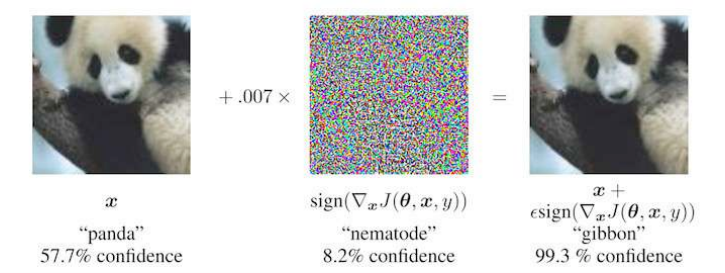
\includegraphics[width=0.7\linewidth]{Images/panda.png}
    \\
    \emph{Figure 15: L'exemple adverse du pandas}
    \\
\end{center}

La formule suivante décrit le cœur de la méthode du signe du gradient rapide:
\[
x' = x + \epsilon \cdot \text{sign}(\nabla_x J(\theta, x, y))
\]
où $\nabla_x J$ est le gradient de la fonction de perte du modèle par rapport au vecteur de pixels d'entrée original $x$, $y$ est le vecteur d'étiquettes véritables pour $x$ et $\theta$ est le vecteur de paramètres du modèle. Du vecteur de gradient (qui a la même longueur que le vecteur des pixels d'entrée), nous avons seulement besoin du signe: le signe du gradient est positif (+1) si une augmentation de l'intensité du pixel augmente la perte (l'erreur que le modèle commet) et négatif (-1) si une diminution de l'intensité du pixel augmente la perte. Cette vulnérabilité se produit lorsque un réseau neuronal traite une relation entre une intensité de pixel d'entrée et le score de classe de manière linéaire. En particulier, les architectures de réseaux neuronaux qui favorisent la linéarité, tels que les LSTM, les réseaux maxout, les réseaux avec des unités d'activation ReLU ou d'autres algorithmes d'apprentissage machine linéaires comme la régression logistique, sont vulnérables à la méthode du signe du gradient rapide. L'attaque est effectuée par extrapolation. La linéarité entre l'intensité du pixel d'entrée et les scores de classe conduit à une vulnérabilité aux valeurs aberrantes.

\subsubsection{Tout est un grille-pain: le patch adversarial}

L'une de mes méthodes préférées apporte des exemples adversaires dans la réalité physique. Brown et al. (2017) ont conçu une étiquette imprimable qui peut être collée à côté des objets pour les faire ressembler à des grille-pains pour un classificateur d'images.

\begin{center}
    \centering
    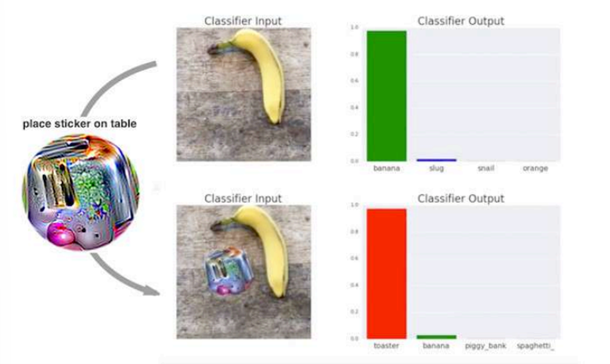
\includegraphics[width=0.7\linewidth]{Images/patch_grille_pain.png}
    \\
    \emph{Figure 15: Le patch grille-pains }
    \\
\end{center}
\\

\subsubsection{Tortue Imprimée en 3D}
La distance attendue sous transformation peut être écrite comme suit :
\[
\mathbb{E}_{t\sim{}T}[d(t(x^\prime),t(x))]
\]
où \( x \) est l'image originale, \( t(x) \) est l'image transformée (par exemple, tournée), \( x' \) est l'exemple adverse et \( t(x') \) sa version transformée.
À part travailler avec une distribution de transformations, la méthode EOT suit le schéma familier de la recherche d'exemples adversaires comme un problème d'optimisation.
Nous essayons de trouver un exemple adverse \( x' \) qui maximise la probabilité pour la classe sélectionnée \( y_t \) (par exemple, "fusil") à travers la distribution des transformations possibles \( T \) :
\[
\arg\max_{x^\prime}\mathbb{E}_{t\sim{}T}[\log{}P(y_t|t(x^\prime))]
\]
Avec la contrainte que la distance attendue sur toutes les transformations possibles entre l'exemple adverse \( x' \) et l'image originale \( x \) reste en dessous d'un certain seuil :
\[
\mathbb{E}_{t\sim{}T}[d(t(x^\prime),t(x))]<\epsilon\quad\text{et}\quad{}x\in[0,1]^d
\]

\begin{center}
    \centering
    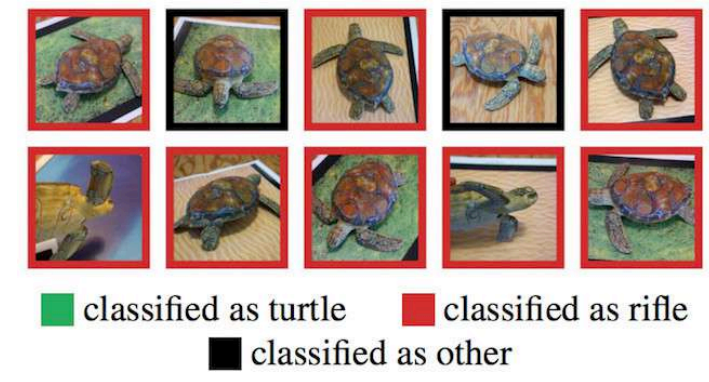
\includegraphics[width=0.7\linewidth]{Images/tortue.png}
    \\
    \emph{Figure 16: La tortue-fusil }
    \\
\end{center}
\\

\subsubsection{L'Adversaire Aveugle : Attaque en Boîte Noire}
Comment cela fonctionne :

\begin{enumerate}
    \item Commencez avec quelques images qui proviennent du même domaine que les données d'entraînement, par exemple, si le classificateur à attaquer est un classificateur de chiffres, utilisez des images de chiffres. La connaissance du domaine est requise, mais pas l'accès aux données d'entraînement.
    \item Obtenez des prédictions pour l'ensemble actuel d'images de la boîte noire.
    \item Entraînez un modèle substitut sur l'ensemble actuel d'images (par exemple, un réseau neuronal).
    \item Créez un nouvel ensemble d'images synthétiques en utilisant une heuristique qui examine pour l'ensemble actuel d'images dans quelle direction manipuler les pixels pour que la sortie du modèle ait plus de variance.
    \item Répétez les étapes 2 à 4 pour un nombre prédéfini d'époques.
    \item Créez des exemples adversaires pour le modèle substitut en utilisant la méthode du gradient rapide (ou similaire).
    \item Attaquez le modèle original avec des exemples adversaires.
\end{enumerate}

L'objectif du modèle substitut est d'approximer les frontières de décision du modèle en boîte noire, mais pas nécessairement d'atteindre la même précision.
Les auteurs ont testé cette approche en attaquant des classificateurs d'images formés sur divers services d'apprentissage machine en nuage. Ces services forment des classificateurs d'images sur des images et des étiquettes téléchargées par l'utilisateur.
Le logiciel entraîne automatiquement le modèle -- parfois avec un algorithme inconnu de l'utilisateur -- et le déploie.
Le classificateur donne ensuite des prédictions pour les images téléchargées, mais le modèle lui-même ne peut pas être inspecté ni téléchargé.
Les auteurs ont pu trouver des exemples adversaires pour divers fournisseurs, jusqu'à 84 \% des exemples adversaires étant mal classifiés.
La méthode fonctionne même si le modèle en boîte noire à tromper n'est pas un réseau neuronal. Cela inclut des modèles d'apprentissage machine sans gradients tels que les arbres de décision.


\subsection{Prototypes et Critiques}
Un prototype est une instance de données représentative de toutes les données. Une critique est une instance de données qui n'est pas bien représentée par l'ensemble des prototypes. Il existe de nombreuses approches pour trouver des prototypes dans les données. L'une d'elles est le k-medoids, un algorithme de clustering lié à l'algorithme des k-means. Tout algorithme de clustering qui retourne de véritables points de données comme centres de clusters serait qualifié pour sélectionner des prototypes. Mais la plupart de ces méthodes ne trouvent que des prototypes, et pas de critiques. Ce chapitre présente MMD-critic de Kim et al. (2016), une approche qui combine des prototypes et des critiques dans un seul cadre.

\subsubsection{Théorie}
La procédure MMD-critic à un haut niveau peut être brièvement résumée :
\begin{enumerate}
    \item Sélectionnez le nombre de prototypes et de critiques que vous souhaitez trouver.
    \item Trouvez des prototypes avec une recherche gloutonne. Les prototypes sont sélectionnés de manière à ce que la distribution des prototypes soit proche de la distribution des données.
    \item Trouvez des critiques avec une recherche gloutonne. Les points sont sélectionnés comme critiques lorsque la distribution des prototypes diffère de celle des données.
\end{enumerate}
Plusieurs éléments sont nécessaires pour trouver des prototypes et des critiques pour un ensemble de données avec MMD-critic. Il nous faut une fonction noyau pour estimer les densités de données, et une mesure qui nous indique à quel point deux distributions sont différentes afin que nous puissions déterminer si la distribution des prototypes sélectionnés est proche de la distribution des données. Cela est résolu en mesurant la divergence maximale de moyenne (MMD). En outre, en fonction de la fonction noyau, nous avons besoin de la fonction témoin pour nous dire à quel point deux distributions sont différentes en un point de données particulier. Avec la fonction témoin, nous pouvons sélectionner des critiques. Le dernier élément est une stratégie de recherche pour de bons prototypes et critiques, ce qui est résolu avec une recherche simple gloutonne.

Un choix pour le noyau est le noyau à base radiale (RBF) :
\[
k(x, x') = \exp\left(-\gamma ||x - x'||^2\right)
\]
où \(||x - x'||^2\) est la distance euclidienne entre deux points et \(\gamma\) est un paramètre d'échelle.

La formule suivante montre comment calculer la mesure MMD carrée (MMD2) :
\[
\text{MMD}^2 = \frac{1}{m^2} \sum_{i,j=1}^m k(z_i, z_j) - \frac{2}{mn} \sum_{i,j=1}^{m,n} k(z_i, x_j) + \frac{1}{n^2} \sum_{i,j=1}^n k(x_i, x_j)
\]
\(k\) est une fonction de noyau qui mesure la similarité entre deux points. \(m\) est le nombre de prototypes \(z\), et \(n\) est le nombre de points de données \(x\) dans notre ensemble de données original. Les prototypes \(z\) sont une sélection de points de données \(x\). Chaque point est multidimensionnel, c'est-à-dire qu'il peut avoir plusieurs variables. L'objectif de MMD-critic est de minimiser MMD2. Plus MMD2 est proche de zéro, mieux la distribution des prototypes correspond aux données.

\subsubsection{Algorithme pour trouver des prototypes}
Nous combinons la mesure MMD2, le noyau et la recherche gloutonne dans un algorithme pour trouver des prototypes :

\begin{itemize}
    \item Commencez avec une liste vide de prototypes.
    \item Tant que le nombre de prototypes est inférieur au nombre \(m\) choisi :
    \begin{itemize}
        \item Pour chaque point dans l'ensemble de données, vérifiez combien MMD2 est réduite lorsque le point est ajouté à la liste des prototypes. Ajoutez le point de données qui minimise MMD2 à la liste.
    \end{itemize}
    \item Retournez la liste des prototypes.
\end{itemize}

\subsection{Fonction témoin}
L'ingrédient restant pour trouver des critiques est la fonction témoin, qui nous indique à quel point deux estimations de densité diffèrent en un point particulier. Elle peut être estimée en utilisant :

\[
\text{témoin}(x) = \frac{1}{n} \sum_{i=1}^n k(x, x_i) - \frac{1}{m} \sum_{j=1}^m k(x, z_j)
\]

Pour trouver des critiques, nous cherchons des valeurs extrêmes de la fonction témoin dans les deux directions, négatives et positives.

\subsection{Explicabilité globale}
En option, nous pouvons utiliser MMD-critic pour rendre n'importe quel modèle d'apprentissage machine globalement explicable en examinant les prototypes et les critiques ainsi que leurs prédictions de modèle. La procédure est la suivante :

\begin{enumerate}
    \item Trouvez des prototypes et des critiques avec MMD-critic.
    \item Entraînez un modèle d'apprentissage machine comme d'habitude.
    \item Prédisez les résultats pour les prototypes et les critiques avec le modèle d'apprentissage machine.
    \item Analysez les prédictions : Dans quels cas l'algorithme s'est-il trompé ?
\end{enumerate}
Vous avez maintenant un certain nombre d'exemples qui représentent bien les données et vous aident à trouver les faiblesses du modèle d'apprentissage machine.


\begin{center}
    \centering
    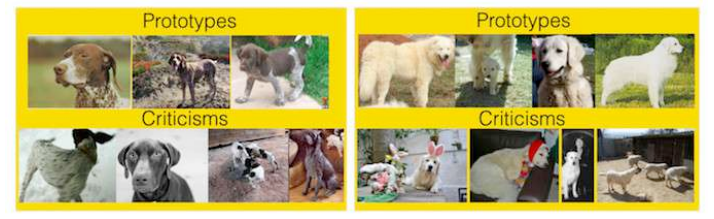
\includegraphics[width=0.7\linewidth]{Images/prototypes_critiques.png}
    \\
    \emph{Figure 17: Prototypes et critiques }
    \\
\end{center}
\\

\subsubsection{Avantages :}
Vous êtes libre de choisir le nombre de prototypes et de critiques. MMD-critic fonctionne avec des estimations de densité des données. Cela fonctionne avec n'importe quel type de données et n'importe quel type de modèle d'apprentissage automatique. L'algorithme est facile à mettre en œuvre.

\subsubsection{Inconvénients :}
Comment sélectionnons-nous un noyau et son paramètre d'échelle? De plus, lorsque nous utilisons MMD-critic comme un classificateur de prototype le plus proche, nous pouvons régler les paramètres du noyau. Il prend toutes les variables en entrée, sans tenir compte du fait que certaines variables pourraient ne pas être pertinentes pour prédire le résultat d'intérêt. Il y a du code disponible, mais il n'est pas encore implémenté sous forme de logiciel bien emballé et documenté.


\subsection{Instances Influentes}

\textbf{Valeur aberrante} : Une valeur aberrante est une instance qui est très éloignée des autres instances dans l'ensemble de données. Lorsqu'une valeur aberrante influence le modèle, il s'agit également d'une instance influente.

\textbf{Instance influente} : Une instance influente est une instance de données dont la suppression a un fort effet sur le modèle entraîné.

Les modèles d'apprentissage automatique sont finalement un produit des données d'entraînement et la suppression d'une des instances d'entraînement peut affecter le modèle résultant. On appelle une instance d'entraînement ``influente'' lorsque sa suppression des données d'entraînement change considérablement les paramètres ou les prédictions du modèle. Ce chapitre vous présente deux approches pour identifier des instances influentes, à savoir les diagnostics de suppression et les fonctions d'influence.


\textbf{Pourquoi les instances influentes aident-elles à comprendre le modèle ?}

L'idée clé derrière les instances influentes pour l'interprétabilité est de retracer les paramètres et les prédictions du modèle jusqu'à leur origine : les données d'entraînement. Avec des instances influentes, nous ne considérons pas le modèle comme fixe, mais comme une fonction des données d'entraînement.

\textbf{Comment trouver des instances influentes ?}

Nous avons deux moyens de mesurer l'influence : notre première option est de supprimer l'instance des données d'entraînement, de réentraîner le modèle sur l'ensemble d'entraînement réduit et d'observer la différence dans les paramètres ou les prédictions du modèle (soit individuellement, soit sur l'ensemble de données complet). La deuxième option est de donner un poids accru à une instance de données en approximant les changements de paramètres basés sur les gradients des paramètres du modèle.

\subsubsection{Diagnostics de Suppression}

DFBETA mesure l'effet de la suppression d'une instance sur les paramètres du modèle. La distance de Cook (Cook, 1977\footnote{Référence}) mesure l'effet de la suppression d'une instance sur les prédictions du modèle. Pour les deux mesures, nous devons réentraîner le modèle à plusieurs reprises, en omettant chaque fois des instances individuelles.

DFBETA est défini comme :

\[
DFBETA_{i}=\beta-\beta^{(-i)}
\]

où \(\beta\) est le vecteur de poids lorsque le modèle est entraîné sur toutes les instances de données, et \(\beta^{(-i)}\) est le vecteur de poids lorsque le modèle est entraîné sans l'instance \(i\).

La distance de Cook a été inventée pour les modèles de régression linéaire et des approximations pour les modèles de régression linéaire généralisée existent. La distance de Cook pour une instance d'entraînement est définie comme la somme (mise à l'échelle) des différences au carré dans le résultat prédit lorsque la \(i\)-ème instance est retirée de l'entraînement du modèle.

\[
D_i=\frac{\sum_{j=1}^n(\hat{y}_j-\hat{y}_{j}^{(-i)})^2}{p\cdot MSE}
\]

où le numérateur est la différence au carré entre la prédiction du modèle avec et sans la \(i\)-ème instance, sommée sur l'ensemble de données.
Le dénominateur est le nombre de caractéristiques \(p\) multiplié par l'erreur quadratique moyenne.
Le dénominateur est le même pour toutes les instances, quelle que soit l'instance \(i\) supprimée.

\textbf{Pouvons-nous utiliser la distance de Cook et DFBETA pour n'importe quel modèle d'apprentissage automatique ?}

DFBETA nécessite des paramètres de modèle, donc cette mesure ne fonctionne que pour les modèles paramétrés.
La distance de Cook ne nécessite aucun paramètre de modèle.
La mesure d'influence la plus simple pour l'effet sur les prédictions du modèle peut être écrite comme suit :

\[
\text{Influence}^{(-i)}=\frac{1}{n}\sum_{j=1}^{n}\left|\hat{y}_j-\hat{y}_{j}^{(-i)}\right|
\]

\subsection{Fonctions d'Influence}

La fonction d'influence est une mesure de la dépendance forte des paramètres du modèle ou des prédictions en fonction d'une instance d'entraînement. Au lieu de supprimer l'instance, la méthode augmente le poids de l'instance dans la fonction de perte par un très petit pas. Cette méthode consiste à approximer la fonction de perte autour des paramètres actuels du modèle en utilisant le gradient et la matrice Hessienne.

L'idée clé derrière les fonctions d'influence est de renforcer la fonction de perte d'une instance d'entraînement par un pas infinitésimalement petit \( \epsilon \), ce qui conduit à de nouveaux paramètres du modèle :

\[
\hat{\theta}_{\epsilon,z}=\arg\min_{\theta{}\in\Theta}(1-\epsilon)\frac{1}{n}\sum_{i=1}^n{}L(z_i,\theta)+\epsilon{}L(z,\theta)
\]

L'intuition derrière cette formule est la suivante : combien la fonction de perte changera-t-elle si nous augmentons le poids d'une instance particulière \( z_i \) des données d'entraînement par un petit \( \epsilon \) et diminuons le poids des autres instances en conséquence ?

La fonction d'influence des paramètres, c'est-à-dire l'influence de l'augmentation du poids de l'instance d'entraînement \( z \) sur les paramètres, peut être calculée comme suit :

\[
I_{\text{up,params}}(z)=\left.\frac{d{}\hat{\theta}_{\epsilon,z}}{d\epsilon}\right|_{\epsilon=0}=-H_{\hat{\theta}}^{-1}\nabla_{\theta}L(z,\hat{\theta})
\]

La dernière expression \( \nabla_{\theta}L(z,\hat{\theta}) \) est le gradient de la perte par rapport aux paramètres pour l'instance d'entraînement renforcée. La première partie \( H^{-1}_{\hat{\theta}} \) est la matrice Hessienne inverse (seconde dérivée de la perte par rapport aux paramètres du modèle). Elle peut être estimée en utilisant :

\[
H_{\theta}=\frac{1}{n}\sum_{i=1}^n\nabla^2_{\hat{\theta}}L(z_i,\hat{\theta})
\]

Plus informellement la matrice Hessienne enregistre la courbure de la perte à un certain point. Le calcul réel de la matrice Hessienne est chronophage si vous avez de nombreux paramètres. Koh et Liang ont suggéré quelques astuces pour le calculer efficacement, ce qui dépasse le cadre de ce chapitre.

\subsubsection{Comment les prédictions changent-elles lorsque nous augmentons le poids de l'instance d'entraînement \( z \) ?}
Nous pouvons soit calculer les nouveaux paramètres et ensuite faire des prédictions en utilisant le modèle nouvellement paramétré, soit calculer directement l'influence de l'instance $z$ sur les prédictions. Pour ce faire, nous utilisons la règle de la chaîne :

\begin{align*}
I_{\text{up,loss}}(z,z_{\text{test}}) &= \left. \frac{d L(z_{\text{test}}, \hat{\theta}_{\epsilon, z})}{d\epsilon} \right|_{\epsilon=0} \\
&= \left. \nabla_{\theta}L(z_{\text{test}}, \hat{\theta})^T \frac{d\hat{\theta}_{\epsilon, z}}{d\epsilon} \right|_{\epsilon=0} \\
&= -\nabla_{\theta}L(z_{\text{test}}, \hat{\theta})^T H^{-1}_{\theta} \nabla_{\theta}L(z, \hat{\theta})
\end{align*}

\begin{itemize}
    \item La première ligne de cette équation signifie que nous mesurons l'influence d'une instance d'apprentissage sur une certaine prédiction $z_{\text{test}}$ comme un changement dans la perte de l'instance de test lorsque nous augmentons le poids de l'instance $z$ et obtenons de nouveaux paramètres $\hat{\theta}_{\epsilon, z}$.
    \item La deuxième ligne de l'équation applique la règle de la chaîne pour obtenir la dérivée de la perte de l'instance de test par rapport aux paramètres, multipliée par l'influence de $z$ sur les paramètres.
    \item Dans la troisième ligne, nous remplaçons l'expression avec la fonction d'influence pour les paramètres. Le premier terme de la troisième ligne, $\nabla_{\theta}L(z_{\text{test}}, \hat{\theta})^T$, est le gradient de l'instance de test par rapport aux paramètres du modèle.
\end{itemize}


\subsubsection{Comprendre le comportement du modèle}

Les différents modèles d'apprentissage automatique ont des manières diverses de faire des prédictions. Même si deux modèles ont la même performance, la manière dont ils font des prédictions à partir des caractéristiques peut être très différente et donc échouer dans des scénarios différents. Comprendre les faiblesses particulières d'un modèle en identifiant des instances influentes aide à former un ``modèle mental'' du comportement du modèle d'apprentissage automatique dans votre esprit. Si vous avez une limite sur le nombre d'instances d'entraînement que vous pouvez vérifier pour la justesse, comment faites-vous une sélection efficace ? La meilleure façon est de sélectionner les instances les plus influentes, car – par définition – elles ont le plus d'influence sur le modèle.

\subsubsection{Avantages et Inconvénients de l'Identification des Instances Influences}

Le processus d'identification des instances influentes en apprentissage automatique a son propre ensemble d'avantages et d'inconvénients.

\paragraph{Avantages}
\\

\begin{enumerate}
    \item \textbf{Compréhension des Données d'Entraînement} : L'identification des instances influentes met en évidence l'importance des données d'entraînement dans le processus d'apprentissage.
    \item \textbf{Outil de Débogage Exceptionnel} : Les fonctions d'influence et les diagnostics de suppression sont parmi les meilleurs outils pour déboguer les modèles d'apprentissage automatique.
    \item \textbf{Universalité} : Les diagnostics de suppression sont agnostiques au modèle, ce qui signifie que cette approche peut être appliquée à n'importe quel modèle.
    \item \textbf{Comparaison de Modèles} : Nous pouvons utiliser ces méthodes pour comparer différents modèles d'apprentissage automatique et mieux comprendre leurs comportements variés, en allant au-delà de la simple comparaison des performances prédictives.
    \item \textbf{Création de Données d'Entraînement Adverses} : Les fonctions d'influence via les dérivées peuvent également être utilisées pour créer des données d'entraînement adverses. Ces instances sont manipulées de telle manière que le modèle ne peut pas prédire certaines instances de test correctement lorsque le modèle est formé sur ces instances manipulées.
\end{enumerate}

\paragraph{Inconvénients}
\\

\begin{enumerate}
    \item \textbf{Coût de Calcul Élevé} : Il est très coûteux de calculer les instances influentes.
    \item \textbf{Limitation des Fonctions d'Influence} : Les fonctions d'influence sont une bonne alternative aux diagnostics de suppression, mais uniquement pour les modèles avec des paramètres différentiables.
    \item \textbf{Approximation} : Les fonctions d'influence ne sont qu'approximatives.
    \item \textbf{Absence de Seuil Clair} : Il n'y a pas de mesure d'influence claire à partir de laquelle on qualifie une instance d'influente ou de non-influente.
    \item \textbf{Suppression Individuelle} : Les mesures d'influence ne prennent en compte que la suppression d'instances individuelles et non la suppression de plusieurs instances à la fois.
\end{enumerate}
